\section{Stabilité numérique}
\subsection{Méthode}
\begin{frame}{Principe}
\begin{itemize}
\item Un schéma d'intégration direct stable:
\begin{equation*}
\exists h_0 > 0 \hspace{0.5cm}\text{such as} \hspace{0.5cm} \forall h \in [0,h_0]
\end{equation*}  
une perturbation finie du vecteur d'état au temps $t_n$ donne une variation non croissante du vecteur d'état à un temps postérieur $t_{n+j}$.

\item Effet de la perturbation au temps $t_{n+1}$:
\begin{equation}
X_{n+1} = H X_n
\end{equation}sera amplifié si les valeurs propre ont un module supérieur à $1$.
\end{itemize}
\end{frame}

\begin{frame}{élément standard}
\begin{itemize}
\item \underline{vecteur d'état:}
\begin{equation}
X^n = \begin{bmatrix}
\dot{u}^n \\
 u^n
\end{bmatrix}, \hspace{1cm} X^{n+1} = \begin{bmatrix}
\dot{u}^{n+1} \\
 u^{n+1}
\end{bmatrix}
\end{equation}
\item \underline{Matrice d'amplification: }
\item équation du mouvement au temps $t_{n}$ et $t_{n+1}$:
\begin{equation}
\begin{cases}
    M  \Ddot{U}^n = -C \Dot{U}^n - K U^n +P_{int}^n \\
    M \Ddot{U}^{n+1} = -C \Dot{U}^{n+1} - K U^{n+1} +P_{int}^{n+1} 
\end{cases}
\end{equation}
\item et la relation de récurrence donnée par la méthode de Newmark:
\begin{equation}
\begin{cases}
\dot{U}_{n+1} = \dot{U}_n + (1-\gamma)dt \ddot{U}_n + \gamma dt \ddot{U}_{n+1} \\
U_{n+1} = U_n +dt \dot{U}_n + dt^2 \left(\frac{1}{2}-\beta\right) \ddot{U}_n + dt^2 \beta \ddot{U}_{n+1}
\end{cases}
\end{equation}
\item H est de taille $8 \times 8$.
\end{itemize}
\end{frame}


\begin{frame}{Elément PML}
\begin{itemize}
\item \underline{Vecteur d'état:}
\begin{equation}
X_n = \begin{bmatrix}
\dot{u}_n \\
u_n \\
\hat{\epsilon}_{n} \\
\hat{E}_{n} \\
\hat{\Sigma}_{n}
\end{bmatrix}, \hspace{1cm}
X_{n+1}= \begin{bmatrix}
\dot{u}_{n+1} \\
u_{n+1} \\
\hat{\epsilon}_{n+1} \\
\hat{E}_{n+1} \\
\hat{\Sigma}_{n+1}
\end{bmatrix}
\end{equation} 

\item \underline{Matrice d'amplification: }
\item équation du mouvement aux temps $t_{n}$ et $t_{n+1}$:
\begin{equation}
\begin{cases}
    M \ddot{u}_n + C \dot{u}_n 
+K u_n + p(\epsilon_{n},E_{n},\Sigma_{n}) = F_{ext} \\
    M \ddot{u}_{n+1} +C \dot{u}_{n+1} 
+K u_{n+1} + p(\epsilon_{n+1},E_{n+1},\Sigma_{n+1}) = F_{ext}
\end{cases}
\end{equation}
\item Et les relations de récurrence donnée par la méthode de Newmark:
\item H a une taille de $52 \times 52$.
\end{itemize}
\end{frame}




\subsection{Results}
\begin{frame}{Stabilité élément 2D}
\begin{itemize}
\item \underline{élément 2D linéaire à 4 noeuds:}
\begin{figure}
\centering
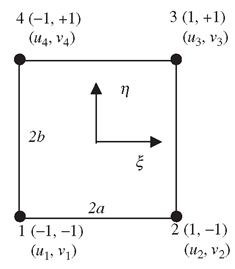
\includegraphics[width=0.4\linewidth]{images/square2d.png}
\end{figure}
\end{itemize}
\end{frame}

\begin{frame}{élément standard: schéma implicite}
\begin{figure}[ht] 
  \label{ fig7} 
  \begin{minipage}[b]{0.5\linewidth}
    \centering
    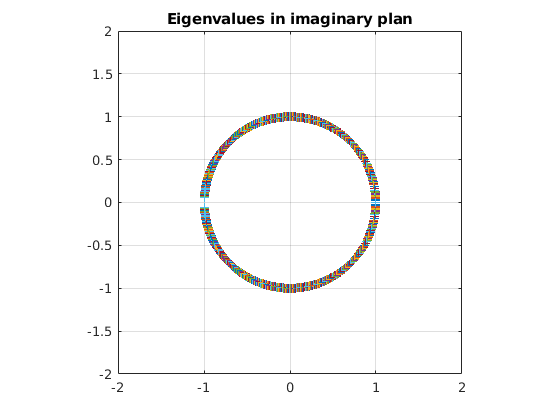
\includegraphics[scale=.35]{images/eig_imp_st.png} \\

  \end{minipage}%%
  \begin{minipage}[b]{0.5\linewidth}
    \centering
    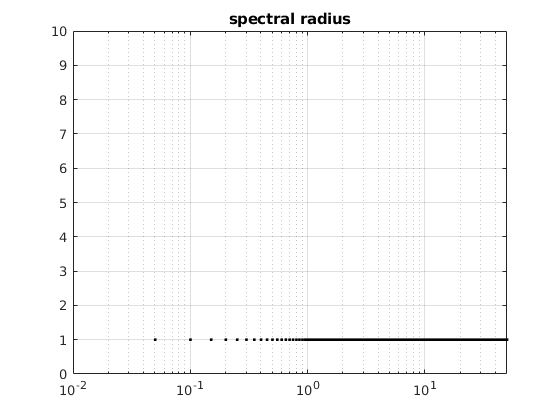
\includegraphics[scale=.35]{images/sr_imp_st.png} \\
  \end{minipage} 
\end{figure}
\begin{itemize}
\item Module des valeurs propres inférieurs à $1$.
\item Le schéma d'intégration pour l'élémént standard est stable.
\end{itemize}
\end{frame}

\begin{frame}{Elément PML: schéma implicite}
\begin{figure}[ht] 
  \label{ fig7} 
  \begin{minipage}[b]{0.5\linewidth}
    \centering
    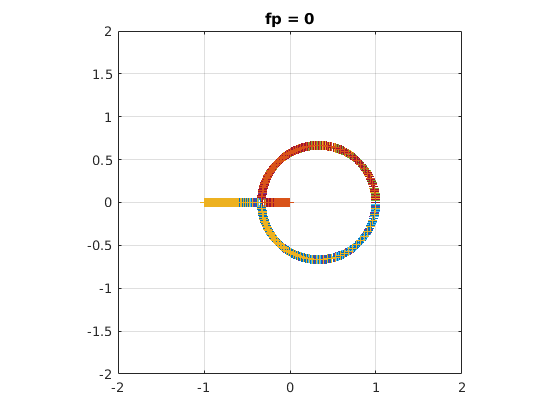
\includegraphics[scale=.34]{images/eig_imp_pml0.png} \\

  \end{minipage}%%
  \begin{minipage}[b]{0.5\linewidth}
    \centering
    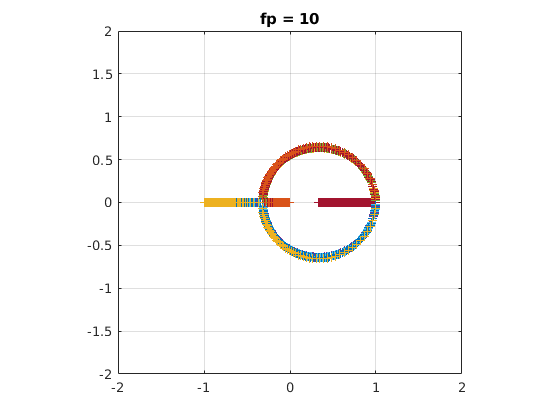
\includegraphics[scale=.34]{images/eig_imp_pml10.png} \\
  \end{minipage} 
  \begin{minipage}[b]{0.5\linewidth}
    \centering
    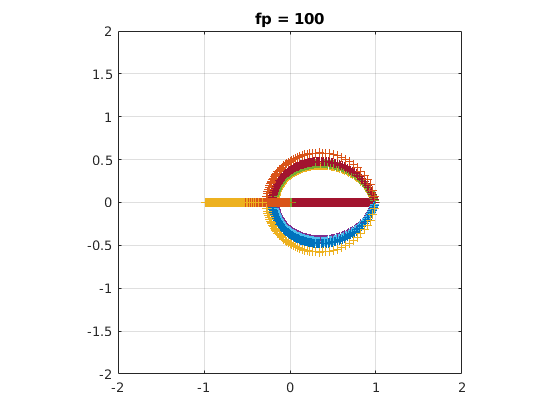
\includegraphics[scale=.34]{images/eig_imp_pml100.png} \\
  \end{minipage}%% 

\end{figure}
\end{frame}

\begin{frame}{Elément PML: schéma implicite}
\begin{figure}[ht] 
  \label{ fig7} 
  \begin{minipage}[b]{0.5\linewidth}
    \centering
    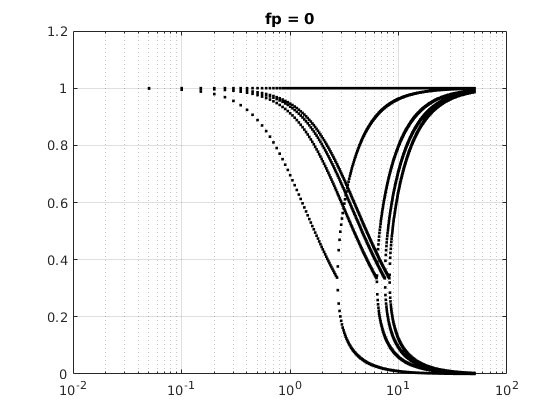
\includegraphics[scale=.34]{images/sr_imp_pml0.png} \\

  \end{minipage}%%
  \begin{minipage}[b]{0.5\linewidth}
    \centering
    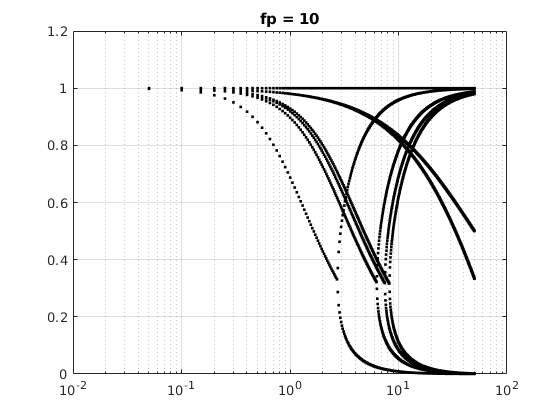
\includegraphics[scale=.34]{images/sr_imp_pml10.png} \\
  \end{minipage} 
  \begin{minipage}[b]{0.5\linewidth}
    \centering
    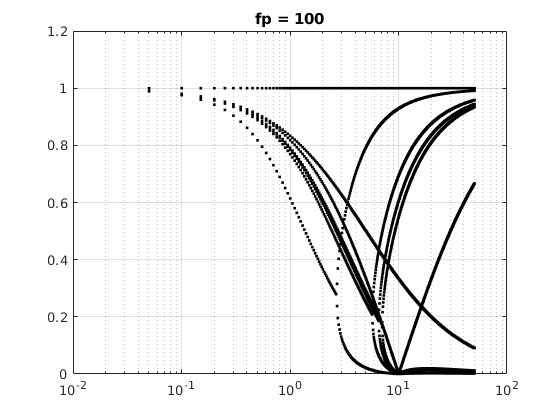
\includegraphics[scale=.34]{images/sr_imp_pml100.png} \\
  \end{minipage} 

\end{figure}
\end{frame}

